% feature selection
% Connor Walsh -  11/2/2014

%Bag-Of-Words and beyond...
Naturally, when presented with a dataset comprised wholly of text strings, the prevailing response is to employ a \emph{Bag-of-words} approach in feature selection in which a dictionary of chosen words or phrases are used to discriminate between multiple document classes. While this feature selection method certainly has merit, the information it conveys is limited due to the loss of structure imposed during feature transformation. For this reason, we incorporate additional features which preserve some syntactic structure in order to exploit our prior knowledge of context-free grammar.

We also implement a series of lexical parsers.  For example, we use NLTK to do part of speech tagging in each sentence for each document sample.  This allows us to track the counts of each tag as a separate feature.  We generate a sentence tree for each sentence.  This allows us to use features that include the depth and breadth of the sentence to judge complexity overall for each document.  One interesting extra feature drawn from this is the ambiguity of noun reference.  When a sentence is referentially ambiguous, two trees are generated.  This allows us to judge the average incidences of referential ambiguity in a document and use this as a feature.  This feature, combined with sentence complexity, should be effective at discriminating between the two classes.  The Corpus used for lexical parsing is the generic Brown Corpus though we plan to experiment with several others.

%Scoring Features
While carefully premeditating the types of features to include in the final learning system is crucial for an accurate classifier, often it is unclear which features will yield optimal performance. For a binary linear discriminant learner, the accuracy of performance manifests itself as the degree of separability between classes of high dimensional features. Thus, it is absolutely critical to evaluate the candidate features with respect to their separability between classes.

To this end, we have developed a method to filter the best features in terms of the information they convey for class discrimination. The method we present draw on previous work and is designed to evaluate generic feature types.
The general idea is to choose features which display a large amount of class imbalance, whether this be in the frequency count per corpus or the number of corpora which contain a given feature. For example,  fig \ref{fg:hists}(a,b) shows a feature (the frequency of the word ``in") with poor separability and a feature (the frequency of the word ``We") with strong separability.

\begin{center}
\begin{tabular}{@{}cc@{}}
\label{fg:hists}
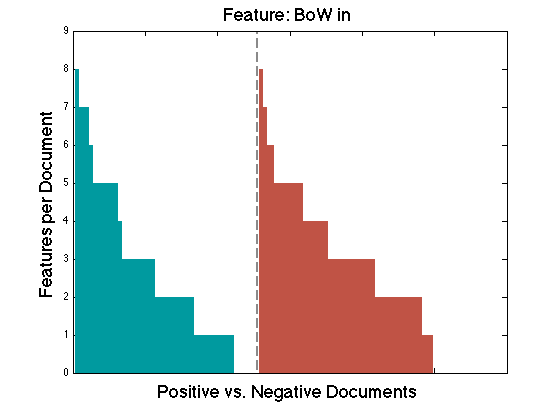
\includegraphics[height=60mm]{figs/features/bad_feature} &
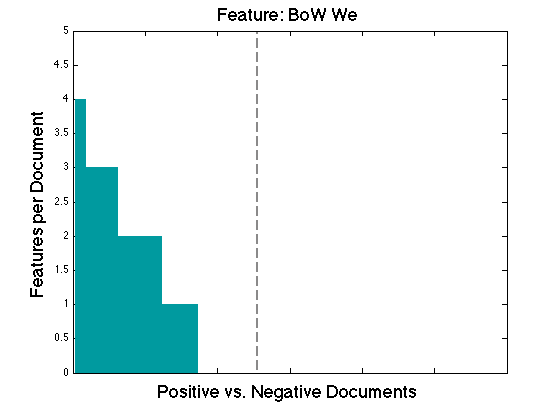
\includegraphics[height=60mm]{figs/features/great_feature} \\
\ref{fg:hists} (a)  & \ref{fg:hists} (b) \\
\end{tabular}
\end{center}

To select for the best features, we formulate the problem as follows,
\begin{eqnarray}
f^{*}_{h} &=& \underset{f}{argmax}\ D_{h}(X^{+}_{f}, X^{-}_{f})\\
f^{*}_{I} &=& \underset{f}{argmax}\ D_{I}(X^{+}_{f}, X^{-}_{f})
\end{eqnarray}

where $f^{*}_{h}$ is the optimal feature which maximizes a hamming distance, $D_h$, between positive and negative training examples, $X^{+}$ and $X^{-}$, transformed by feature $f$. Similarly, $f^{*}_{I}$ is the optimal feature which maximizes an intersection distance, $D_{I}$. 

For $D_{h}$ we define the distance as follows,
\begin{eqnarray}
D_h = \sum |X^{+}_{\{x>0\}} - X^{-}_{\{x>0\}}|
\end{eqnarray}
which is the absolute valued distance between binary vectors, $X^{+}_{\{x>0\}}$ and  $X^{-}_{\{x>0\}}$,  which indicate whether each document has a non-zero feature count or not.
For $D_{I}$ we use the tanimoto distance. Both distance measures return values in $[ 0, 1 ]$.

In addition to using the distance measures to choose the most appropriate features, we also use the values in a weighting scheme employed by our feature transform. We define the feature transform as follows,
\begin{eqnarray}
f_{h} &=& sign(max(X^{+}, X{-})) \cdot exp(a_0 D_h)/a_1 \\
f_{I} &=& sign(max(X^{+}, X{-})) \cdot exp(b_0 D_{I})/b_1
\end{eqnarray}
where the constants ($a_0,a_1,b_0,b_1$) are chosen. This transform provides weights which increase exponentially as the distances grow and ensure that the weights have the proper sign corresponding to the class imbalance of the feature. Fig \ref{fg:weights}(c) shows an example of the feature transform function.
\begin{center}
\begin{tabular}{@{}c@{}}
\label{fg:weights}
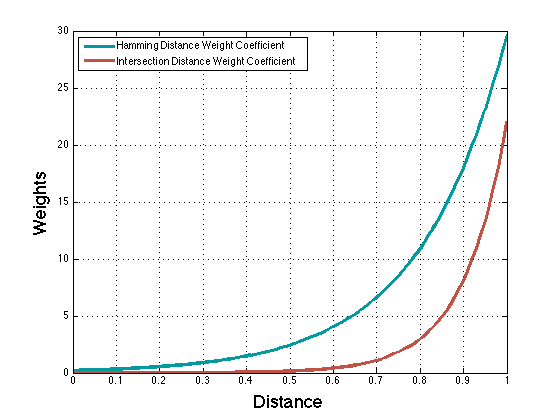
\includegraphics[height=60mm]{figs/features/weightScheme} \\
\ref{fg:weights}(c)\\
\end{tabular}
\end{center}
